\documentclass[12pt,a4paper]{article}

\usepackage[czech]{babel}
\usepackage{csquotes}
\usepackage{graphicx}
\usepackage{textcomp}
\usepackage{caption}
\usepackage{biblatex}
\addbibresource{bibliography.bib}

% rovnice zarovnávat doleva
\usepackage[fleqn]{amsmath}

% neodsazovat nové odstavce
\setlength{\parindent}{0pt}


\begin{document}

%%%%%%%%%%%%%%%% TITLE PAGE %%%%%%%%%%%%%%%%
\begin{titlepage}
\begin{center}

\includegraphics[width=0.5\linewidth]{img/logo.pdf}
\vspace{3cm}

\LARGE\uppercase{Modelování a simulace 2021/2022}
\vspace{1cm}

\LARGE\textbf{Simulační studie na technologii Vehicle-to-grid}

\vspace*{\fill}
\large{Ondřej Mach (xmacho12)}

\large{Rostislav Lán (xlanro00)}

\end{center}
\end{titlepage}


%%%%%%%%%%%%%%%% TABLE OF CONTENTS %%%%%%%%%%%%%%%%
\pagenumbering{arabic}
\setcounter{page}{1}
\tableofcontents
\clearpage

%%%%%%%%%%%%%%%% THE ACTUAL DOCUMENT %%%%%%%%%%%%%%%%

\section{Úvod}
Tato práce pokládá otázku, zda je technologie Vehicle-to-grid ekonomicky rentabilní.
Přínos této technologie je posouzen podle simulačního modelu, který modeluje výrobu a spotřebu elektrické energie v rámci domu.
Technologie je poměrně nová a studie na toto téma dochází k různým závěrům, což bylo motivací pro vytvoření tohoto projektu.

\subsection{Technologie Vehicle-to-grid}
Vehicle to Grid (V2G) je technologie využívající vozidla schopná vyrábět nebo uchovávat elektrickou energii (např. elektrická, hybridní nebo vodíková vozidla).
Vyžaduje datové spojení mezi vozidlem a nabíjecí stanicí, umožňující monitorovat stav sítě a podle něj modifikovat množství nabíjené elektřiny.
Umožňuje nečinným vozidlům zapojeným do sítě napájet část nebo celou domácnost anebo dodávat do této sítě v baterii uloženou elektřinu.
Tím může pomoci redukovat domácnosti využívající tento systém výdaje za elektřinu a také může snížit zatížení sítě.
V rámci tohoto procesu však dochází k opotřebení baterie, tudíž snížení životnosti vozidla.

\subsection{Režimy Vehicle-to-grid}
Systém V2G může být nakonfigurován více způsoby.
V1G, neboli jednosměrné V2G, je režim, kdy vozidlo nemůže dodávat do sítě elektřinu,
je však schopno určit nejvhodnější časy pro nabíjení ze sítě. To mu umožňuje významně snížit cenu nabíjení, zátěž sítě a využívat větší podíl elektřiny z obnovitelných zdrojů.
V2B/V2H, neboli vehicle-to-building/home, při tomto režimu je vozidlo schopné omezeně dodávat uloženou energii do budovy/domácnosti v případě fluktuace napští v síti, nebo při výpadcích proudu.
V2X, jinak také vehicle-to-everything, režim zamšřený na komunikaci s ostatními vozidly nebo infrastrukturou, primárním účelem není kontrola nabíjení, ale efektivita a bezpečnost dopravy.
V2G - vehicle-to-grid, nebo bi-directional smart charging. Umožňuje dodávat vyráběnou/uchovávanou elektřinu zpět do sítě a tím snížit její zatížení.

\subsection{Předchozí studie}

\section{Simulační model}
Simulační model je logicky rozdělen na domácnost, solární elektrárnu, elektrické vozidlo a měřící zařízení.

\bigskip
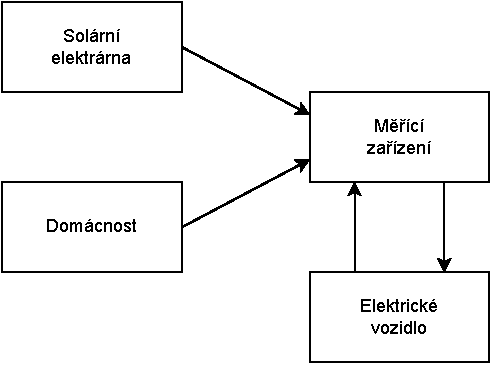
\includegraphics[width=0.5\linewidth]{img/diagram.pdf}
\bigskip

V rámci solární elektrárny je náhodně generován výkon.
Ten je závislý pouze na modelovém čase, ze kterého je určeno roční období.

Modul domácnosti generuje spotřebovaný výkon, který je také závislý na čase,


\subsection{Solární elektrárna}
V rámci tohoto modulu je náhodně generována výroba energie.
Jediným výstupem je tudíž proměnná, ve které je uložen výkon elektrárny v daném čase.
Vstupem pro toto generování je čas, podle kterého je určeno roční období.
To má v realitě významný vliv na výkon elektrárny, proto je nutné ho brát v úvahu.

Konkrétními faktory, které mají významný vliv na výrobu elektřiny jsou délka dne, pozice slunce vůči panelu a počasí.
Tady napsat, jak se počítá výkon podle období.


\subsection{Domácnost}
Modul domácnosti má za úkol náhodně modelovat spotřebu elektrické energie tak,
aby se co nejblíže podobal reálné domácnosti.
Má tedy jedinou výstupní proměnnou, která udává výkon spotřebovaný v daném čase.
Spotřeba domácnosti závisí na čase, ze kterého je spočítán den v týdnu a roční období.

Spotřeba v domácnosti je zcela nezávislá na výkonu elektrárny v daném čase.
Zde by mohl být drobný rozdíl oproti realitě.
Členové domácnosti mohou záměrně spotřebovávat více elektřiny, pokud má zrovna elektrárna přebytečný výkon.
Dobrý příklad tohoto by bylo zapnutí elektrické trouby, když je elektrárna v provozu.

\subsubsection{Implementace}
Domácnost je modelována jako proces knihovny SIMLIB.
Spotřeba je počítána jako součet konstantní a dynamické spotřeby.
Konstantní představuje výkon, který je odebírán vždy.
V reálné domácnosti by tento výkon představovaly například síťové modemy a switche.
Dále je do této části započítána pohotovostní spotřeba televizí, monitorů, počítačů a jiných spotřebičů.

Dynamická spotřeba představuje spotřebiče, které spotřebovávají energii pouze občas.
Toto je naprostá většina spotřebičů používaných v domácnosti.
Patřila by sem například varná konvice, elektrický sporák, televize, počítač a mnoho dalších.
Každý spotřebič má zadáno, mezi kterými časy se spouští a jaký podíl této doby je průměrně aktivní. [TODO mozna i neco dalsiho]
Podle těchto parametrů náhodně generuje zátěž.

Dynamická spotřeba je zcela nutná, aby byl model validní.
V případě, že by byla modelována pouze konstantní spotřeba,
celková spotřeba by mohla být stejná, ale spotřeba ze sítě resp. dodávka do sítě by se výrazně lišila.

Modul domácnosti periodicky sčítá výkon všech spotřebičů, který je monitorován monitorovacím zařízením.
Tato spotřeba je zobrazena na obrázku ~\ref{fig:load_power},
kde jedna křivka představuje okamžitou spotřebu a druhá šestihodinový pohyblivý průměr.

\begin{figure}
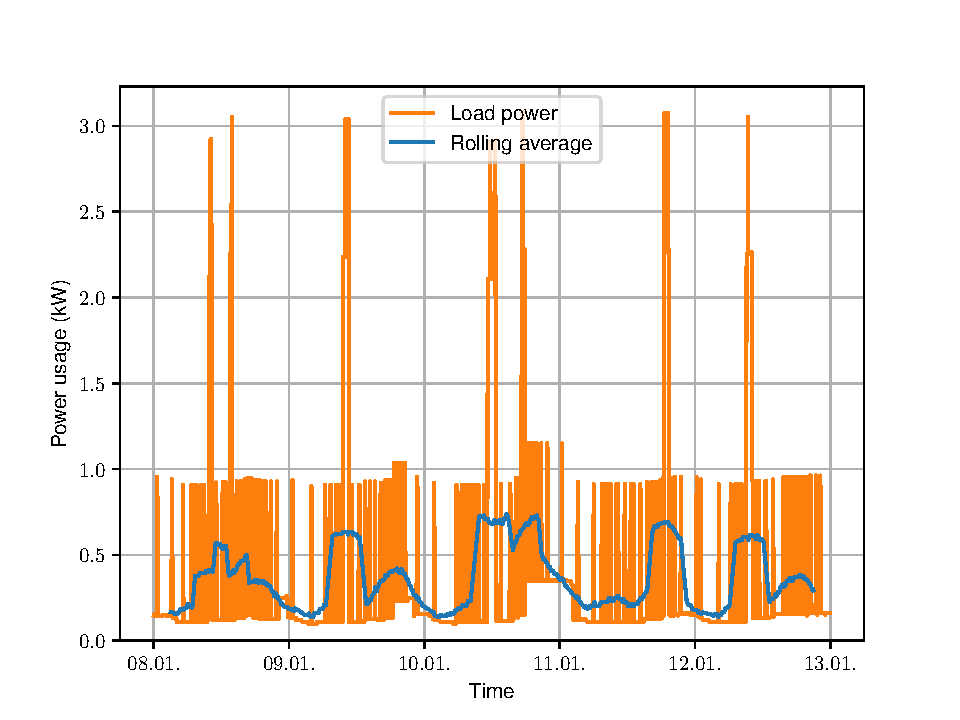
\includegraphics[width=\linewidth]{img/load_power.pdf}
\caption{Spotřeba domácnosti v rozsahu 5 dní}
\label{fig:load_power}
\end{figure}

\subsubsection{Spotřebiče}
Všechny spotřebiče jsou implementovány jako C++ objekty, přičemž jejich třídy vždy dědí ze třídy \texttt{Load}.
Rozhraní \texttt{Load} poskytuje metodu \texttt{readPower}, která vrací současný výkon spotřebiče.
Díky ní mohou být všechny odečítány modulem domácnosti.
Spotřebiče jsou implementovány třídami \texttt{Appliance} a \texttt{LightBulb}.

Spotřebiče třídy \texttt{Appliance} mají jako parametry výkon, průměrný čas běhu a pravděpodobnosti, že budou zapnuté pro každou hodinu.
Pravděpodobnosti jsou implementovány jako pole 24 položek typu float,
každá z nich určuje pravděpodobnost, že bude daný spotřebič v tu hodinu aktivní.
Konkrétní hodnoty byly převzaty ze studie. \cite{TORRITI201737}

Žárovky třídy \texttt{LightBulb} jsou implementovány tak,
že

\subsubsection{Verifikace modelu}

Pro ověření správné spotřeby v závislosti na čase byl sestrojen histogram,
který zobrazuje průměrnou spotřebu v každé hodině dne (Obrázek \ref{fig:average_day_load}).
Data jsou zprůměrována z 1 simulovaného roku roku.
Implementovaný model víceméně koresponduje s předlohou \cite{TORRITI201737}.

Celá domácnost spotřebuje 3.27 MWh za rok, což zhruba odpovídá průměrné spotřebě domácnosti v České Republice\cite{CEZ}.



\begin{figure}
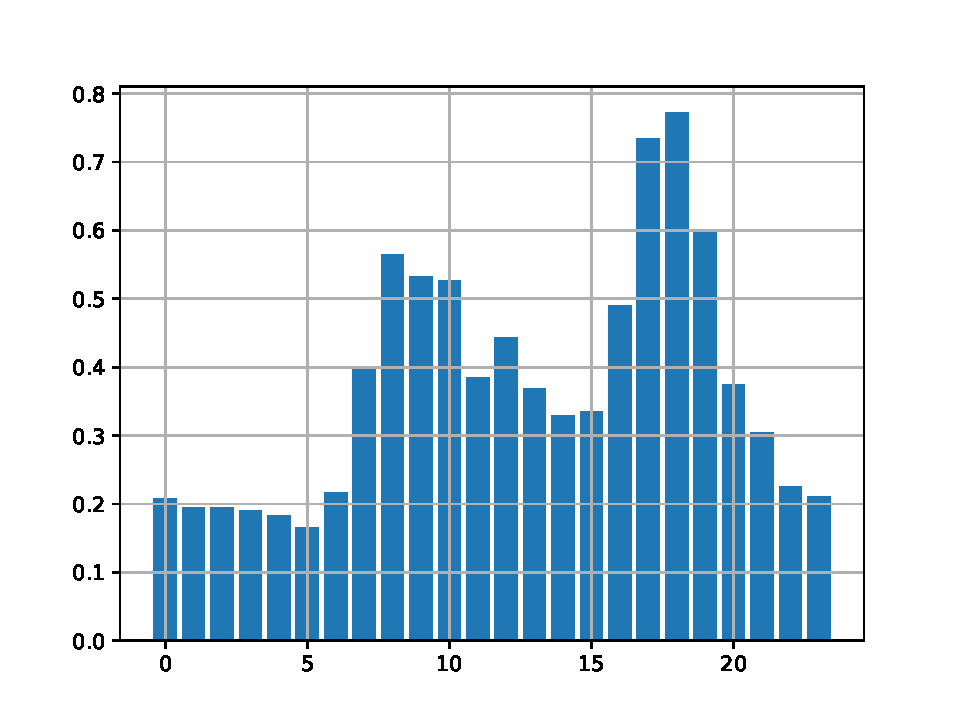
\includegraphics[width=\linewidth]{img/average_day_load.pdf}
\caption{Průměrná spotřeba domácnosti v závislosti na čase}
\label{fig:average_day_load}
\end{figure}

\subsection{Elektrické vozidlo}
Elektrické vozidlo je implementováno jako další proces knihovny SIMLIB.
V porovnání s realitou tento modul obsahuje více, než jen EV.
Obsahuje i nabíjecí stanici, která nabíjí vozidlo, případně dodává energii do sítě.
V tomto modulu jsou také počítány veškeré ztráty energie, ke kterým dochází při nabíjení, resp. vybíjení.

Tento modul může být nastaven na více režimů operace, a těmi jsou V2G, V1G, obyčejná nabíječka a žádné auto.
Režim V2G znamená, že EV se nabíjí podle toho, jestli je nějaký přebytek energie z elektrárny.
Dále v tomto režimu EV dodává elektřinu do sítě, pokud ho o to měřící zařízení požádá.
Může tak pokrýt spotřebu v domu, pokud zrovna elektrárna nedodává dostatený výkon.

V režimu V1G je zachováno nabíjení, které spotřebuje pouze přebytek energie v síti.
Oproti V2G ale EV nemůže dodávat energii do sítě.

V režimu obyčejné nabíječky EV nebere žádný ohled na současnou spotřebu v síti.
Nabíjí se konstantní rychlostí, dokud není baterie plná.

Modul také obsahuje režim, který představuje, že žádné EV není připojeno k síti.
Jedná se spíše o implementační detail, díky kterému lze simulaci provést i bez EV.

Nabíjení vozidla a dodávání energie do sítě je implementováno metodami třídy v C++.
Objekt EV má proměnnou, ve které je současná energie, která je nabita v baterii.
Měřící nástroj může vozidlu poslat, že chce v následujícím měřícím úseku nabít do baterie nějaké množství energie.
Tato funkce vrátí skutečné množství energie, které bylo spotřebované vozidlem.
Pokud je množství energie za daný čas příliš velké,
vozidlo se nemůže nabíjet tak rychle, spotřebuje pouze množství omezené maximálním výkonem nabíječky.
Dodávka energie do sítě se řídí stejným pravidlem.

Pokud je EV na minimálním limitu baterie, nedodává již žádnou energii do sítě.
Pokud je naopak baterie plně nabitá, vozidlo nespotřebovává žádnou energii.

\subsection{Měřící zařízení}
Měřící zařízení je implementováno jako proces knihovny SIMLIB.
Tento proces provádí v pravidelných intervalech měření spořeby a výroby elektrické energie.
Pokud toto zařízení zjistí nadbytek energie v síti, dá EV možnost tuto energii spotřebovat.
Pokud je v síti naopak nedostatek energie a bylo by nutné ji brát od dodavatele, požádá EV o dodávku energie.
Poté spočítá sumu i s elekrickým vozidlem.
Všechny naměřené údaje jsou ukládány do sdíleného pole, aby šly přečíst a analyzovat po skončení simulace.

\section{Provedení simulace}

\subsection{Nastavení parametrů}

\subsection{Získaná data}


\section{Závěr}

Provedená simulace dokázala, že ...

\printbibliography

\end{document}


















































